\begin{figure}
\centering
\begin{minipage}{0.45\textwidth}
\centering
\begin{tikzpicture}[font=\small]
\pgfmathsetmacro{\r}{2.5}
\pgfmathsetmacro{\A}{30}
\pgfmathsetmacro{\B}{180-\A}
\pgfmathsetmacro{\C}{\B-\A}
\fill[lgray,opacity=0.5]([shift={(\A:0.4*\r)}]0,0) arc (\A:\B:0.4*\r)--++(\B:0.3*\r) arc (\B:\A:0.7*\r)--cycle;
\fill[lgray,opacity=0.5]([shift={(\A+0.2*\C:0.3*\r)}]0,0) arc (\A+0.2*\C:\B:0.3*\r)--++(\B:0.1*\r) arc (\B:\A+0.2*\C:0.4*\r)--cycle;
\fill[lgray,opacity=0.5]([shift={(\A+0.4*\C:0.2*\r)}]0,0) arc (\A+0.4*\C:\B-0.2*\C:0.2*\r)--++(\B-0.2*\C:0.1*\r) arc (\B-0.2*\C:\A+0.4*\C:0.3*\r)--cycle;
\fill[lgray,opacity=0.5]([shift={(\A:0.7*\r)}]0,0) arc (\A:\A+0.2*\C:0.7*\r)--++(\A+0.2*\C:0.1*\r) arc (\A+0.2*\C:\A:0.8*\r)--cycle;
\fill[gray,opacity=0.5]([shift={(\A+0.2*\C:0.5*\r)}]0,0) arc (\A+0.2*\C:\A+0.4*\C:0.5*\r)--++(\A+0.4*\C:0.1*\r) arc (\A+0.4*\C:\A+0.2*\C:0.6*\r)--cycle;
\draw[-latex](-1.1*\r,0)node[left]{$\theta=\pi$}--(1.1*\r,0)node[right]{$\theta=0$};
\draw([shift={(0:\r)}]0,0) arc (0:180:\r)node[pos=0.07,right]{$r=a$};
\draw(0,0)--++(\A:1.1*\r)coordinate[pos=0.3](kRA)coordinate[pos=0.8](kRB)node[right]{$\theta=\beta$};
\draw(0,0)--++(\B:1.1*\r)coordinate[pos=0.25](kLA)coordinate[pos=0.7](kLB)node[left]{$\theta=\alpha$};
\foreach \k in {0.1,0.2,0.3,0.4,0.5,0.6,0.7,0.8,0.9}{\draw([shift={(\A:\k*\r)}]0,0) arc (\A:\B:\k*\r);}
\foreach \kk in {0.2,0.4,0.6,0.8}{\draw(0,0)--++(\A+\kk*\C:\r);}
\draw(\A+0.2*\C:\r+0.1)--++(\A+0.2*\C:0.4);
\draw(\A+0.4*\C:\r+0.1)--++(\A+0.4*\C:0.4);
\draw[stealth-stealth]([shift={(\A+0.2*\C:\r+0.3)}]0,0) arc (\A+0.2*\C:\A+0.4*\C:\r+0.3)node[pos=0.4,above]{$\Delta \theta$};
\draw([shift={(\A-0.05*\C:0.5*\r)}]0,0) arc (\A-0.05*\C:\A-0.15*\C:0.5*\r)coordinate[pos=0.5](kL);
\draw([shift={(\A-0.05*\C:0.6*\r)}]0,0) arc (\A-0.05*\C:\A-0.15*\C:0.6*\r)coordinate[pos=0.5](kH);
\draw[stealth-](kL)--++(\A-0.1:-0.2);
\draw[stealth-](kH)--++(\A-0.1:0.3)node[right,xshift=-0.75ex]{$\Delta r$};
\draw(\A+0.3*\C:0.55*\r)node[circ]{}node[pin={[pin distance=0.25cm]170:{$(r_k,\theta_k)$}}]{}node[pin={[pin distance=0.3cm]0:{$\Delta S_k$}}]{};
\draw[thick](kLA)to[out=-10,in=160]coordinate[pos=0.35](Ga)(kRA);
\draw[thick](kLB) to [out=80,in=130]coordinate[pos=0.20](Gb)(kRB);
\draw(Ga)node[pin=-135:{$r=g_1(\theta)$}]{};
\draw(Gb)node[pin=135:{$r=g_2(\theta)$}]{};
\end{tikzpicture}
\caption{
خطہ \عددی{R:\, g_1(\theta)\le r\le g_2(\theta)}، \عددی{\alpha\le \theta\le \beta}  پنکھا نما خطہ \عددی{Q:\, 0\le r\le a}، \عددی{\alpha\le \theta\le \beta}  میں پایا جاتا ہے۔ خطہ \عددی{Q} کی خانہ بندی شعاعوں اور دائری قوسین سے کرتے ہوئے \عددی{R} کی خانہ بندی کی جاتی ہے۔
}
\end{minipage}\hfill
\begin{minipage}{0.45\textwidth}
\centering
\begin{tikzpicture}[font=\small]
\pgfmathsetmacro{\ra}{2.5}
\pgfmathsetmacro{\rb}{\ra+1}
\pgfmathsetmacro{\angA}{30}
\pgfmathsetmacro{\angB}{55}
\pgfmathsetmacro{\angC}{1/2*(\angA+\angB)}
\pgfmathsetmacro{\rc}{1/2*(\ra+\rb)}
\pgfmathsetmacro{\rd}{1.15*\rb}
\draw(0,0)node[below left]{$O$}--++(\angA:\ra) arc (\angA:\angB:\ra)--(0,0);
\draw[fill=lgray](\angA:\ra)--(\angA:\rb) arc (\angA:\angB:\rb)--(\angB:\ra)node[pos=0.35,shift={(\angB+90:0.25)}]{$\Delta r$} arc (\angB:\angA:\ra);
\draw[decorate,decoration={brace,amplitude=10pt,raise=3pt}](\angA:\rb)--(0,0)node[pos=0.5,shift={(\angA-90:0.75)}]{\text{\RL{بڑا خطہ}}};
\draw[decorate,decoration={brace,amplitude=10pt,raise=3pt}](0,0)--++(\angB:\ra)node[pos=0.5,shift={(\angB+90:0.80)}]{\text{\RL{چھوٹا  خطہ}}};
\draw(\angA:\rb+0.1*\rb)--++(\angA:0.1*\rb);
\draw(\angB:\rb+0.1*\rb)--++(\angB:0.1*\rb);
\draw[stealth-stealth]([shift={(\angA:\rd)}]0,0) arc (\angA:\angB:\rd)node[pos=0.5,shift={(\angC:0.3)}]{$\Delta \theta$};
\draw(\angC:\rc)node[circ]{}node[shift={(\angC+90:0.3)}]{$r_k$}node[shift={(\angC-90:0.35)}]{$\Delta S_k$};
\draw[thick](0,0)--++(\angC:\rb)node[circ]{}node[pin={[pin distance=1cm]100:{$r_k+\tfrac{\Delta r}{2}$}}]{};
\draw(\angC:\ra)node[circ]{}node[pin={[pin distance=1.25cm]115:{$r_k-\tfrac{\Delta r}{2}$}}]{};
\end{tikzpicture}
\caption{
سایہ دار خطے کا رقبہ \عددی{\Delta S_k} حاصل کرنے کے لئے بڑے خطے سے چھوٹے خطے  کا رقبہ منفی کریں۔
}
\end{minipage}
\end{figure}

%========================================

\begin{figure}
\centering
\begin{subfigure}{0.45\textwidth}
\centering
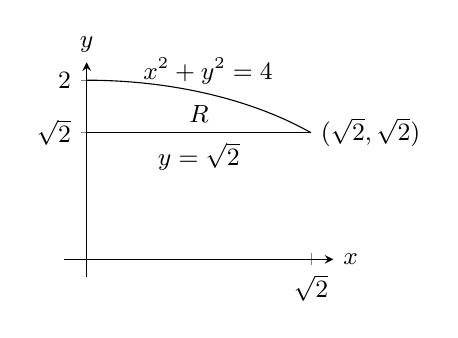
\begin{tikzpicture}[font=\small,declare function={f(\x)=sqrt(4-\x^2);}]
\pgfmathsetmacro{\k}{sqrt(2)}
\begin{axis}[clip=false,width=5cm,axis lines=middle,xtick={\k},ytick={\k,2},xticklabels={$\sqrt{2}$},yticklabels={$\sqrt{2}$,$2$},xmin=0,ymin=0,enlargelimits=true, xlabel={$x$}, ylabel={$y$}, xlabel style={at={(current axis.right of origin)},anchor=west},ylabel style={at={(current axis.above origin)},anchor=south}]
\addplot[domain=0:sqrt(2)]{f(x)}node[pos=0.5,above]{$x^2+y^2=4$};
\addplot[]coordinates{(0,\k)(\k,\k)}node[pos=0.5,below]{$y=\sqrt{2}$}node[right]{$(\sqrt{2},\sqrt{2})$}node[pos=0.5,above]{$R$};
\end{axis}
\end{tikzpicture}
\end{subfigure}\hfill
\begin{subfigure}{0.45\textwidth}
\centering
\begin{tikzpicture}[font=\small,declare function={f(\x)=sqrt(4-\x^2);}]
\pgfmathsetmacro{\k}{sqrt(2)}
\pgfmathsetmacro{\ang}{60}
\pgfmathsetmacro{\ra}{sqrt(2)/(sin(\ang))}
\begin{axis}[clip=false,width=5cm,axis lines=middle,xtick={\k},ytick={\k,2},xticklabels={$\sqrt{2}$},yticklabels={$\sqrt{2}$,$2$},xmin=0,ymin=0,enlargelimits=true, xlabel={$x$}, ylabel={$y$}, xlabel style={at={(current axis.right of origin)},anchor=west},ylabel style={at={(current axis.above origin)},anchor=south}]
\addplot[domain=0:sqrt(2)]{f(x)};
\addplot[]coordinates{(0,\k)(\k,\k)}node[pos=0.5,above]{$R$};
\draw[-latex](0,0)--(\ang:2.5)node[right]{$L$};
\draw(\ang:\ra)node[pin=-45:{\text{\RL{شعاع \عددی{\sqrt{2}\csc\theta} پر داخل ہوتی ہے}}}]{};
\draw(\ang:2)node[pin={[above]100:{\text{\RL{شعاع \عددی{r=2} پر خارج ہوتی ہے}}}}]{};
\draw[-stealth]([shift={(0:0.5)}]0,0) arc (0:\ang:0.5)node[pos=0.6,right]{$\theta$};
\end{axis}
\end{tikzpicture}
\end{subfigure}
\begin{subfigure}{1\textwidth}
\centering
\begin{tikzpicture}[font=\small,declare function={f(\x)=sqrt(4-\x^2);}]
\pgfmathsetmacro{\k}{sqrt(2)}
\pgfmathsetmacro{\ang}{60}
\pgfmathsetmacro{\ra}{sqrt(2)/(sin(\ang))}
\begin{axis}[clip=false,width=5cm,axis lines=middle,xtick={\k},ytick={\k,2},xticklabels={$\sqrt{2}$},yticklabels={$\sqrt{2}$,$2$},xmin=0,ymin=0,ymax=2.25,enlargelimits=true, xlabel={$x$}, ylabel={$y$}, xlabel style={at={(current axis.right of origin)},anchor=west},ylabel style={at={(current axis.above origin)},anchor=south}]
\addplot[domain=0:sqrt(2)]{f(x)};
\addplot[]coordinates{(0,\k)(\k,\k)}node[pos=0.5,above]{$R$};
\draw[-latex](0,0)--(\ang:2.5)node[right]{$L$};
\draw[-stealth]([shift={(0:0.5)}]0,0) arc (0:45:0.5)node[pos=0.6,right]{\text{\RL{کم سے کم \عددی{\theta}}}};
\draw[dashed](0,0)--(45:2.5)node[right]{$y=x$};
\draw(0,2.2)node[pin=20:{\RL{زیادہ سے زیادہ زاویہ \عددی{\tfrac{\pi}{2}} ہے}}]{};
\end{axis}
\end{tikzpicture}
\end{subfigure}
\end{figure}


%==============
\begin{figure}
\centering
\begin{tikzpicture}[font=\small,declare function={f(\x)=1+cos(\x);}]
\pgfmathsetmacro{\ang}{-40}
\pgfmathsetmacro{\ra}{1+cos(\ang)}
\begin{axis}[axis on top,axis equal,clip=false,width=5cm,axis lines=middle,xtick={1,2},xticklabels={\rlap{$1$},\rlap{$2$}},ytick={\empty},enlargelimits=true, xlabel={$x$}, ylabel={$y$}, xlabel style={at={(current axis.right of origin)},anchor=west},ylabel style={at={(current axis.above origin)},anchor=south}]
\addplot[opacity=0.5,fill=lgray,data cs=polar,domain=0:360,smooth]{f(x)}node[pos=0.2,above right]{$r=1+\cos\theta$};
\draw[fill=white](0,0) circle (1);
\addplot[data cs=polar,domain=90:270,smooth]{f(x)};
\draw[-latex](0,0)--(\ang:2.2);
\addplot[-stealth,domain=0:\ang] ({0.4*cos(x)},{0.4*sin(x)})node[pos=0.6,right]{$\theta$}; 
\draw(\ang:\ra)node[pin={[right]20:{\text{\RL{خارج \عددی{r=1+\cos\theta}}}}}]{};
\draw(\ang:1)node[pin={[below,pin distance=1cm]-110:{\text{\RL{داخل \عددی{r=1}}}}}]{};
\draw(0,1)node[pin=135:{$\theta=\tfrac{\pi}{2}$}]{};
\draw(0,-1)node[pin=-135:{$\theta=-\tfrac{\pi}{2}$}]{};
\end{axis}
\end{tikzpicture}
\end{figure}

%======================
\begin{figure}
\centering
\begin{tikzpicture}[font=\small,declare function={f(\x)=sqrt(4*cos(2*\x));}]
\pgfmathsetmacro{\ang}{20}
\pgfmathsetmacro{\ra}{sqrt(4*cos(2*\ang))}
\begin{axis}[axis equal,axis on top,clip=false,width=5cm,axis lines=middle,xtick={\empty},ytick={\empty},enlargelimits=true, xlabel={$x$}, ylabel={$y$}, xlabel style={at={(current axis.right of origin)},anchor=west},ylabel style={at={(current axis.above origin)},anchor=south}]
\addplot[opacity=0.5,fill=lgray,data cs=polar,domain=0:90,smooth]{f(x)};
\addplot[data cs=polar,domain=90:360,smooth]{f(x)}node[pos=0.9,below right]{$r^2=4\cos 2\theta$};
\draw[-latex](0,0)--(\ang:2.5);
\draw(\ang:\ra)node[pin={[above,pin distance=1cm]70:{\text{\RL{خارج \عددی{r=\sqrt{4\cos 2\theta}}}}}}]{};
\draw(0,0)node[pin={[below,pin distance=1cm]-130:{\text{\RL{داخل \عددی{r=0}}}}}]{};
\draw(0,0)--(45:1.25)node[above]{$\tfrac{\pi}{4}$};
\draw(0,0)--(-45:1.25)node[below]{$-\tfrac{\pi}{4}$};
\end{axis}
\end{tikzpicture}
\caption{
تکمل کی قیمت کے حصول میں ہم \عددی{r} کو \عددی{0} تا \عددی{\sqrt{4\cos 2\theta}} جبکہ \عددی{\theta} کو 0 تا \عددی{\tfrac{\pi}{4}} لیتے ہیں۔
}
\end{figure}

%=====================
\begin{figure}
\centering
\begin{minipage}{0.45\textwidth}
\centering
\begin{tikzpicture}[font=\small,declare function={fx(\x)=cos(\x);fy(\x)=sin(\x);}]
\begin{axis}[axis equal,axis on top,clip=false,width=5cm,axis lines=middle,xtick={1},ytick={1},enlargelimits=true, xlabel={$x$}, ylabel={$y$}, xlabel style={at={(current axis.right of origin)},anchor=west},ylabel style={at={(current axis.above origin)},anchor=south}]
\addplot[domain=0:90,smooth]({fx(x)},{fy(x)})node[pos=0.5,right,align=center]{$x^2+y^2=1$\\ $r=1$}node[pos=0,pin=45:{$\theta=0$}]{}node[pos=1,pin=45:{$\theta=\tfrac{\pi}{2}$}]{};
\draw(0,0)node[below left]{$O$};
\end{axis}
\end{tikzpicture}
\caption{
قطبی محدد میں یہ خطہ \عددی{0\le r\le 1}، \عددی{0\le\theta\le\tfrac{\pi}{2}} ہے۔
}
\end{minipage}\hfill
\begin{minipage}{0.45\textwidth}
\centering
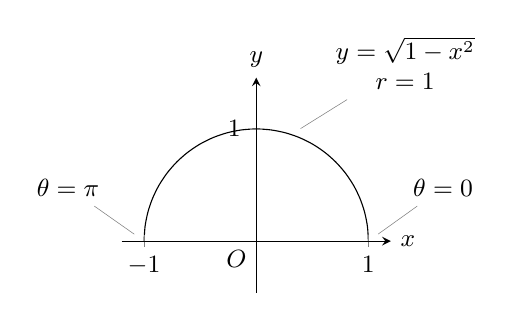
\begin{tikzpicture}[font=\small,declare function={fx(\x)=cos(\x);fy(\x)=sin(\x);}]
\begin{axis}[axis equal,axis on top,clip=false,width=5cm,axis lines=middle,xtick={-1,1},ytick={1},enlargelimits=true, xlabel={$x$}, ylabel={$y$}, xlabel style={at={(current axis.right of origin)},anchor=west},ylabel style={at={(current axis.above origin)},anchor=south}]
\addplot[domain=0:180,smooth]({fx(x)},{fy(x)})node[pos=0.4,pin={[align=center]45:{$y=\sqrt{1-x^2}$\\  $r=1$}}]{}node[pos=0,pin=45:{$\theta=0$}]{}node[pos=1,pin=135:{$\theta=\pi$}]{};
\draw(0,0)node[below left]{$O$};
\end{axis}
\end{tikzpicture}
\caption{
نصف دائری  خطہ \عددی{0\le r\le 1}، \عددی{0\le \theta\le \pi} ہے۔
}
\end{minipage}
\end{figure}

%============

\begin{figure}
\centering
\begin{subfigure}{0.45\textwidth}
\centering
\begin{tikzpicture}[font=\small]
\pgfmathsetmacro{\angA}{-170}
\pgfmathsetmacro{\angB}{100}
\pgfmathsetmacro{\angC}{-10}
\pgfmathsetmacro{\angD}{-135}
\pgfmathsetmacro{\angE}{-100}
\pgfmathsetmacro{\angF}{-40}
\draw[-latex,name path=kx](0,0)--++(-1.5,-1.5)node[left]{$x$};
\draw[-latex](0,0)--++(3,0)node[right]{$y$};
\draw[-latex](0,0)--++(0,2)node[left]{$z$};
\draw[fill=lgray,draw=black,text=black,opacity=0.5](2.5,-0.25)coordinate(kA) to [out=\angA,in=\angB]node[pos=0.75,above left,yshift=-1ex]{$y=g_1(x)$}++(-1.5,-0.75)coordinate(kB)node[above right,xshift=1ex,yshift=0.5ex]{$R$} to [out=\angC,in=\angD]node[pos=0.5,right]{$y=g_2(x)$}(kA);
\path[dashed](kA)--++(0,2.25)coordinate(kC)coordinate[pos=0.5](kE);
\path[dashed](kB)--++(0,3)coordinate(kD)coordinate[pos=0.5](kF);
\draw[dashed](kA)--(kE)  (kB)--(kF);
\draw(kC)--(kE)  (kD)--(kF);
\draw[dashed](kE) to [out=\angA,in=\angB](kF);
\draw(kF) to [out=\angC,in=\angD](kE); 
\draw(kE) to [out=\angE,in=\angF]coordinate[pos=0.25](kLower)(kF);
\draw(kC) to [out=110,in=60]coordinate[pos=0.25](kUpper)(kD);
\draw[](kC) to [out=-\angA,in=-\angB](kD);
\draw[dashed](kD) to [out=-\angC,in=-\angD](kC);
\draw(kLower)node[pin={[right]-10:{$z=f_1(x,y)$}}]{};
\draw(kUpper)node[pin=35:{$z=f_2(x,y)$}]{};
\draw($(kC)!0.5!(kE)$)node[right]{$D$};
\path[name path=kLa](kA)--++(-3.5,0);
\path[name path=kLb](kB)--++(-2.5,0);
\draw[dashed,name intersections={of=kx and kLa}] (kA)--(intersection-1)node[left]{$a$};
\draw[dashed,name intersections={of=kx and kLb}] (kB)--(intersection-1)node[left]{$b$};
\end{tikzpicture}
\end{subfigure}\hfill
\begin{subfigure}{0.45\textwidth}
\centering
\begin{tikzpicture}[font=\small]
\pgfmathsetmacro{\angA}{-170}
\pgfmathsetmacro{\angB}{100}
\pgfmathsetmacro{\angC}{-10}
\pgfmathsetmacro{\angD}{-135}
\pgfmathsetmacro{\angE}{-100}
\pgfmathsetmacro{\angF}{-40}
\draw[-latex,name path=kx](0,0)--++(-1.5,-1.5)node[left]{$x$};
\draw[-latex](0,0)--++(3,0)node[right]{$y$};
\draw[-latex](0,0)--++(0,2)node[left]{$z$};
\draw[fill=lgray,draw=black,text=black,opacity=0.5](2.5,-0.25)coordinate(kA) to [out=\angA,in=\angB]node[pos=0.5, left,xshift=-2ex,yshift=-1ex]{$y=g_1(x)$}++(-1.5,-0.75)coordinate(kB)node[above right,xshift=1ex,yshift=0.5ex]{$R$} to [out=\angC,in=\angD]node[pos=0.75,right]{$y=g_2(x)$}(kA);
\path[dashed](kA)--++(0,2.25)coordinate(kC)coordinate[pos=0.5](kE);
\path[dashed](kB)--++(0,3)coordinate(kD)coordinate[pos=0.5](kF);
%\draw[dashed](kA)--(kE)  (kB)--(kF);
\draw(kC)--(kE)  (kD)--(kF);
\draw[dashed](kE) to [out=\angA,in=\angB](kF);
\draw(kF) to [out=\angC,in=\angD](kE); 
\draw(kE) to [out=\angE,in=\angF]coordinate[pos=0.25](kLower)(kF);
\draw(kC) to [out=110,in=60]coordinate[pos=0.25](kUpper)(kD);
\draw[](kC) to [out=-\angA,in=-\angB](kD);
\draw[dashed](kD) to [out=-\angC,in=-\angD](kC);
\draw($(kC)!0.5!(kE)$)node[right]{$D$};
\path[name path=kLa](kA)--++(-3.5,0);
\path[name path=kLb](kB)--++(-2.5,0);
\draw[dashed,name intersections={of=kx and kLa}] (kA)--(intersection-1)node[left]{$a$};
\draw[dashed,name intersections={of=kx and kLb}] (kB)--(intersection-1)node[left]{$b$};
\draw($(kA)!0.5!(kB)$)node[circ]{}node[pin=-45:{$(x,y)$}]{}--($(kE)!0.5!(kF)+(0,-0.3)$)coordinate(kMm)node[circ]{};
\draw[dashed](kMm)node[pin={[right,pin edge={-,solid},align=center,pin distance=1cm]30:{\text{\RL{داخل}}\\ $z=f_1(x,y)$}}]{}--($(kC)!0.5!(kD)$)node[circ]{}node[pin={[align=center,pin edge={-,solid}]35:{\text{\RL{خارج}}\\ $z=f_2(x,y)$}}]{};
\draw[-latex]($(kC)!0.5!(kD)$)--++(0,1)node[left]{$M$};
\end{tikzpicture}
\end{subfigure}
\begin{subfigure}{1\textwidth}
\centering
\begin{tikzpicture}[font=\small]
\pgfmathsetmacro{\angA}{-170}
\pgfmathsetmacro{\angB}{100}
\pgfmathsetmacro{\angC}{-10}
\pgfmathsetmacro{\angD}{-135}
\pgfmathsetmacro{\angE}{-100}
\pgfmathsetmacro{\angF}{-40}
\draw[-latex,name path=kx](0,0)--++(-1.5,-1.5)node[left]{$x$};
\draw[-latex](0,0)--++(3,0)node[right]{$y$};
\draw[-latex](0,0)--++(0,2)node[left]{$z$};
\draw[name path=kR,fill=lgray,draw=black,text=black,opacity=0.5](2.5,-0.25)coordinate(kA) to [out=\angA,in=\angB]++(-1.5,-0.75)coordinate(kB)node[above right,xshift=1ex,yshift=-0.25ex]{$R$} to [out=\angC,in=\angD](kA);
\path[dashed](kA)--++(0,2.25)coordinate(kC)coordinate[pos=0.5](kE);
\path[dashed](kB)--++(0,3)coordinate(kD)coordinate[pos=0.5](kF);
%\draw[dashed](kA)--(kE)  (kB)--(kF);
\draw(kC)--(kE)  (kD)--(kF);
\draw[dashed](kE) to [out=\angA,in=\angB](kF);
\draw(kF) to [out=\angC,in=\angD](kE); 
\draw(kE) to [out=\angE,in=\angF]coordinate[pos=0.25](kLower)(kF);
\draw(kC) to [out=110,in=60]coordinate[pos=0.25](kUpper)(kD);
\draw[](kC) to [out=-\angA,in=-\angB](kD);
\draw[dashed](kD) to [out=-\angC,in=-\angD](kC);
\draw($(kC)!0.5!(kE)$)node[right]{$D$};
\path[name path=kLa](kA)--++(-3.5,0);
\path[name path=kLb](kB)--++(-2.5,0);
\draw[dashed,name intersections={of=kx and kLa}] (kA)--(intersection-1)node[left]{$a$};
\draw[dashed,name intersections={of=kx and kLb}] (kB)--(intersection-1)node[left]{$b$};
\draw($(kA)!0.5!(kB)$)coordinate(kLM)node[circ]{}node[pin=-100:{$(x,y)$}]{}--($(kE)!0.5!(kF)+(0,-0.3)$)coordinate(kMm)node[circ]{};
\draw[dashed](kMm)--($(kC)!0.5!(kD)$)node[circ]{};
\draw[-latex]($(kC)!0.5!(kD)$)--++(0,1)node[left]{$M$};
\path[name path=kL](kLM)--++(-3,0);
\draw[-latex,name intersections={of=kL and kx}](intersection-1)--++(3.5,0)node[right]{$L$};
\path[name path=kLeft](kLM)--(intersection-1);
\path[name path=kRight](kLM)--++(1.5,0);
\draw[name intersections={of=kLeft and kR}](intersection-1)node[pin={[align=center]-120:{\text{داخل}\\$y=g_1(x)$}}]{};
\draw[name intersections={of=kRight and kR}](intersection-1)node[pin={[align=center]-60:{\text{خارج}\\  $y=g_2(x)$}}]{};
\end{tikzpicture}
\end{subfigure}
\end{figure}

%==========================

\begin{figure}
\centering
\begin{tikzpicture}[font=\small]
\pgfmathsetmacro{\ra}{1.5}
\pgfmathsetmacro{\rb}{1/2*\ra}
\pgfmathsetmacro{\h}{1.25}
\pgfmathsetmacro{\ang}{15}
\pgfmathsetmacro{\angY}{-30}
\pgfmathsetmacro{\angO}{-60}
\pgfmathsetmacro{\angI}{-180-\angO+\ang}
\pgfmathsetmacro{\angOO}{110}
\pgfmathsetmacro{\angII}{135}
\pgfmathsetmacro{\angOa}{110-180}
\pgfmathsetmacro{\angIa}{-135}
\pgfmathsetmacro{\angOb}{180-135}
\pgfmathsetmacro{\angIb}{-180}
\pgfmathsetmacro{\angOc}{0}
\pgfmathsetmacro{\angIc}{-90}
\draw[-latex](\ang:2)--++(\ang:-4)node[left]{$x$};
\draw[-latex,name path=ky](0,0)--++(\angY:1.25)node[right]{$y$};
\draw[name path=kc,rotate=\ang](0,0) circle (\ra cm and \rb cm);
\draw(\ang:-\ra)coordinate(kLleft)--++(0,\h)coordinate(kHleft) (\ang:\ra)coordinate(KLright)--++(0,\h)coordinate(kHright)++(-0.3,-0.2)coordinate(kNear);
\draw(kHleft) to [out=\angO,in=180+\ang] (0,0) to [out=\ang,in=\angI](kHright);
\draw(kHleft) to [out=\angOO,in=\angII](kHright);
\path[name intersections={of=kc and ky}](intersection-1)++(0,\h+0.5)coordinate(kHmid);
\draw(kHleft) to [out=\angOa,in=\angIa] (kHmid)to [out=\angOb,in=\angIb](kNear) to [out=\angOc,in=\angIc](kHright);
\draw[dashed](kHright) to [out=170,in=0](0,1.5*\h) to [out=180,in=110](kHleft);
\end{tikzpicture}
\end{figure}

